\documentclass{article}

%usepackages
\usepackage[utf8]{inputenc}
\usepackage{graphicx}
\usepackage[normalem]{ulem}
\usepackage{enumitem}
\usepackage{amsmath}
\usepackage[english]{babel}
\usepackage{amssymb}
\usepackage{amsthm}
\usepackage{hyperref}
\usepackage{pgf,tikz,pgfplots}
\pgfplotsset{compat=1.15}
\usepackage{mathrsfs}
\usetikzlibrary{arrows}
\usepackage[english]{babel}
\usepackage[letterpaper, portrait, margin=1.2in]{geometry}
%\usepackage{fancyhdr}

%new commands
\newcommand{\R}{\mathbb{R}}
\newcommand{\N}{\mathbb{N}}
\newcommand{\Q}{\mathbb{Q}}
\newcommand{\Z}{\mathbb{Z}}
\newcommand{\C}{\mathbb{C}}
\newcommand{\inv}{^{-1}}
\newcommand{\img}{\textmd{Im}\:}
\newcommand{\cok}{\textmd{coker}}
\newcommand{\conv}{\textmd{conv}}
\newcommand{\vertices}{\textmd{vert}}
\newcommand{\st}{\textmd{ s.t. }}
\newcommand{\fracfield}{\textmd{frac}\:}

%new theorem environments
%plain
\theoremstyle{plain}
\newtheorem{thm}{Theorem}[section]
\newtheorem{lemma}[thm]{Lemma}
\newtheorem*{FLH}{Fundamental Lemma of Homology}
%definitions
\theoremstyle{definition}
\newtheorem{definition}{Definition}[section]
\newtheorem{example}{Example}[section]

%remarks
\theoremstyle{remark}

\newtheorem{remark}{Remark}[section]
%title
\title{Summary}
\author{Luca Bracone}
%TODO: add abstract. 
\begin{document}
	\maketitle
	\section{Basic Machine Learning}
	\subsection{Neural Networks}
	\begin{definition}[Perceptron]
		A \emph{Perceptron} is a function $ p:\R^n \to \R $ given by 
		\[ p(x_1, \dots , x_n) = g \left( w_0 + \sum_{i=1}^{n} w_i x_i \right)  \]
		Where $ w_1, \dots, w_n \in \R $ are called the \emph{weights} of $p$, $w_0$ is called the \emph{bias}, and $g:\R \to \R $ is any non-linear function called the \emph{activation}.
		Most of the time we use \[ g(x)=\frac{e^x}{e^x+1} \] the sigmoid function.
	\end{definition}
%	\begin{minipage}{0.3\textwidth}
%			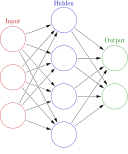
\includegraphics[width=72px]{figure1.png}
%	\end{minipage}
%\begin{minipage}{0.7\textwidth}
	\begin{definition}[Artificial Neural Network]
		A (forward-feeding) \emph{Artificial Neural Network} (ANN) is a function $T: \R^n \to \R^m$ that can be decomposed as such \[ T= l_k \circ \dots \circ l_1  \] Where the $l_i : \R^{n_j} \to \R^{n_{j+1}}$ are called \emph{layers} and are just vectors of perceptrons \[ l_i(\vec{x})=(p_{i,1}(\vec{x}),\dots,p_{i,n_j}(\vec{x})) \].
		In the context of neural networks perceptrons are also called nodes.
	\end{definition}
%\end{minipage}
For some ANN, $T$ and some input $ (x_1,...,x_n) $, we have a desired output $ (y_1,...,y_n) $ we would like $ T $ to match. Denote $ (\hat{y}_1,...,\hat{y}_m) $ the output $T$ actually produced.
\begin{definition}[Loss Function]
	 The \emph{loss} (or sometimes also called \emph{cost}) of $T$ for this input is a function that measures the "distance" between the produced and desired output. For most basic applications, the loss is defined as the $l_2$ norm on $\R^n$
	\[\mathcal{L}(W; x)= \sum_{i=1}^{m} ||y_i - \hat{y}_i||_2^2  \]
\end{definition}
\begin{definition}[Empirical Loss]
	For a set of inputs $X=\{(x_1^1,\dots,x_n^1), \dots , (x_1^m,\dots ,x_n^m)\}$, and $T$ a NN, the \emph{Empirical Loss} is defined as
	\[ J(W)=\frac{1}{|X|} \sum_{\vec{x}\in X} \mathcal{L}(W;x) \]
	the average loss over $X$.
\end{definition}

\subsection{Gradient Descent}
	Any neural network is defined by the weights of its perceptrons. Therefore, in order to have the neural network behave as desired (namely being as close as possible to the desired outputs) one has to find an efficient way to tweak the weights such that the empirical loss becomes as low as possible, when tested on some new inputs. Applying this algorithm repeatedly is called training, and allows us to find a local minimum of the loss function.
	\subsubsection{Gradient Descent}
		 The algorithm of gradient descent involves taking a step in the "right" direction until we reach a stopping condition, most of the time it is when the steps we are taking are too short. Consider $ \frac{\partial J}{\partial w_i} $ where $w_i$ is any weight in $T$, this expression represents how big of a change in $J$ we’ll obtain by moving $w_i$. For each weight $w_i$ in $T$, we denote the vector $ \left(\frac{\partial J}{\partial w_i} \right)_{i\in I} $ as $\nabla J$. The gist of the algorithm revolves around updating the weights $W \gets W - \eta \nabla J$. Where $\eta$ is a constant that has to be well chosen. If too small, gradient descent stops when it meets the slightest uphill, and thus misses a better minimum which might be close by. If too big, gradient descent can only take giant steps and diverges to infinity.


		In practice, calculating the derivative to some particular weight is quite simple, consider the following neural net: \\ \\
		\begin{minipage}{0.55\linewidth}

		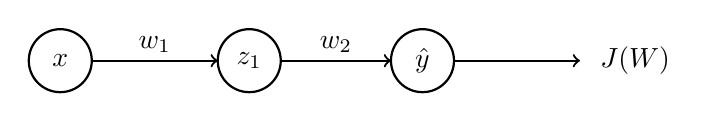
\begin{tikzpicture}
		\draw[thick] (0,0) circle [radius=0.4];
		\node at (0,0) {$x$};
		\draw[->, thick] (0.4,0) -- (2,0);
		\node at (1.2,0.2) {$w_1$};
		\draw[thick] (2.4,0) circle [radius=0.4];
		\node at (2.4,0) {$z_1$};
		\draw[->, thick] (2.8,0) -- (4.2,0);
		\node at (3.5,0.2) {$ w_2 $};
		\draw[thick] (4.6,0) circle [radius=0.4];
		\node at (4.6,0) {$ \hat{y} $};
		\draw[->,thick] (5,0)--(6.6,0);
		\node at (7.3,0) {$ J(W) $};
		\end{tikzpicture}
		\end{minipage}
	\begin{minipage}{0.45\linewidth}
		It's just an application of the chain rule:
		\begin{align*}
		\frac{\partial J}{\partial w_2} &=\frac{\partial J}{\partial \hat{y}} \frac{\partial \hat{y}}{\partial w_2} \\
		\frac{\partial J}{\partial w_1} &= \frac{\partial J}{\partial \hat{y}}\frac{\partial \hat{y}}{\partial z_1}\frac{\partial z_1}{\partial w_1}
		\end{align*}
	\end{minipage}

	Since calculating $\nabla J$ is computationally intensive, consider taking a random subset of your data, and applying gradient descent to it instead. The convergence is going to be more erratic, depending on the size of the subset chosen.
	\subsection{Overfitting}
	When training our neural network, it might happen that it essentially "learns the dataset by heart" making it unable to properly tackle on never seen before data points. There are a few methods to avoid such a problem:
		\begin{figure}[ht!]
		\centering
		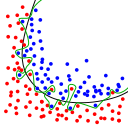
\includegraphics{overfitting.png}
		\caption[image of overfitting]{A parabola+noise is being misunderstood as a complicated winding line \protect \footnotemark}
		\end{figure}
		\footnotetext{Courtesy of wikimedia foundation \href{https://commons.wikimedia.org/wiki/File:Overfitting.svg}{https://commons.wikimedia.org/wiki/File:Overfitting.svg}}
		
	\emph{Dropout} involves randomly setting some nodes to zero during training. This makes the network not rely too much on some path.
	\emph{early stopping} is the process by which after each application of gradient descent, one tests the network. If it performs worse than it did previously, stop the training process.	
	
	\section{Simplicial Complexes}
	\begin{definition}[Convex Hull]
	Let $ u_0,...,u_k \in \R^n $ their \emph{convex hul}l is
	  \begin{equation} 
	  \label{conv-hull}
	  \conv \{u_0,...,u_k\} = \left\{ x= \sum_{i=0}^{n} \lambda_i u_i \ \st    \sum_{i=0}^{n} \lambda_i = 1; \ \lambda_i > 0 \ \forall i \right\} 
	  \end{equation}
	\end{definition}
	
	\begin{definition}[Affinitely Independent, $k$-Simplex]
		Let $u_0,...,u_k \in \R^n$ . They are said to be \emph{affinitely independent }if any point in their convex hull, when written as in ~\eqref{conv-hull} is uniquely written as such.
		In that case instead of convex hull, we speak of \emph{$k$-simplex}.
	\end{definition}
	
	\begin{definition} [Faces and Cofaces]
		Let $ \{u_{i_0},...,u_{i_m} \} \subseteq \{u_0,...,u_k\} $ we say that $ \tau = \conv\{u_{i_1},...,u_{i_m}\} $ is a \emph{face} of $ \sigma = \conv\{u_1,..,u_k\} $ which we write $ \tau < \sigma $. Equivalently $ \sigma $ is a \emph{co-face} of $ \tau $.
	\end{definition}
	
	\begin{definition}[Simplicial Complex]
		A \emph{simplicial complex} $K$ is a collection of simplices such that:
		\begin{enumerate}[label=(S\arabic*)]
			\item $ \forall \sigma \in K, \ \tau < \sigma \implies \tau \in K $. 
			\item $ \forall \sigma,\tau \in K, \ \sigma \cap \tau $ is either empty or a face.
		\end{enumerate}
		
	The \emph{dimension} of $K$ is $ \dim K = \max_{\sigma \in K} \dim \sigma $ and the dimension of a $k$-simplex is $k$.
	The \emph{underlying space} of $K$, $|K|$ is the topological space $ \bigcup_{\sigma \in K} \sigma $ with the subspace topology.
	\end{definition}
%todo:add examples of complexes
\begin{definition}[Triangulation]
	Let $X$ be a topological space and $K$ a simplicial complex, if there exists a homeomorphism $ \phi : X \to |K| $ we say that $X$ is triangulable. In that case the couple $ (K,\phi) $ is called a triangulation of $X$
\end{definition}

	\begin{definition}[sub-Complex]
		A subset $L \subseteq K$ is a \emph{subcomplex} of K, if it is itself a complex. It is called full if it contains all vertices of $K$.
	\end{definition}
	
	\begin{example}[Skeleton]
		The \emph{$j$-skeleton} of a simplicial complex $K$ is $K^{(j)}= \{ \sigma \in K \st \dim\sigma \leq j \} \subseteq K $. In particular the 0-skeleton is called $\vertices(K)$ and it consists of the vertices of $K$
	\end{example}
	
	\begin{definition}[Star and Link]
		Let $K$ be a simplicial complex and pick $ \sigma \in K $. Its \emph{star}, $ st\sigma = \{ \tau \in K \st \tau < \sigma \} $. unfortunately it's not a sub-complex of $K$ because it's not closed under taking faces. For that we define the \emph{closed star }$ \overline{st}\sigma $ the smallest sub-complex that contains the star.
		%todo explain this better
		Similarly, the \emph{link} of a simplex $ lk\sigma = \{ \tau \in \overline{st}\sigma \st \tau \cap \sigma = \emptyset \} $ the set of simplices in the closed star that don't touch $\sigma$
	\end{definition}
	
	\begin{definition}[Simplicial Maps and Homeomorphisms]
		Let $K$, $L$ be two simplicial complexes and $ \phi: \vertices K \to \vertices L $ a map such that vertices of every simplex in $K$ gets mapped to a vertex of a simplex in $L$, in that case $\phi$ is called a \emph{vertex map}.The map $f: |K| \to |L|$ defined by $ \sum_{i=0}^n \lambda_i u_i \mapsto \sum_{i=0}^n \lambda_i \phi(u_i) $ is called a \emph{simplicial map}. If $ \phi $ is bijective and $ \phi\inv $ is also a vertex map, we call it instead \emph{simplicial homeomorphism}.
	\end{definition}

	\section{Simplicial Homology}
	\begin{definition}[p-Chain]
		Let $K$ be a simplicial complex. A \emph{$ p $-chains} is a formal sum of $p$-simplices of $K$ over a field: \[ c = \sum_{i=1}^{n} a_i \sigma_i \]
	\end{definition}
	For the time being, the field in question is $ \mathbb{F}_2 $. Componentwise addition: $ c + d = \sum_{i=1}^n (c_i + d_i) \sigma_i $ makes the set of $p$-chains into a commutative group which we note as $ (C_p, +) $.
\begin{definition}[Boundary]
	the \emph{Boundary} of a $ p $-simplex is a map $ \partial_p : C_p \to C_{p-1} $ which for a $p$-simplex returns the sum of the $ (p-1) $-faces: \[ \partial_p \sigma = \sum_{j=1}^n [u_1, \dots , \hat{u_j} , \dots , u_p] \]
	where $[ u_1 \dots u_p ]$ is the $p$-simplex given by the convex hull of the $\{u_1, \dots , u_p\}$ and $\hat{u}_j$ means we omit the $j$-th term from that notation.
	This definition extends by linearity to the $p$-chains: \[ \partial_p c = \sum_{i=1}^{n} a_i \ \partial_p\sigma_i  \]
\end{definition}

Turns out $ \partial_p : C_p \to C_{p-1} $ is a group homomorphism. for a simplicial complex $K$ we define its chain complex:
\[\mathcal{C}_K: \ \dots \longrightarrow C_p \stackrel{\partial_p}{\longrightarrow} C_{p-1} \stackrel{\partial_{p-1}}{\longrightarrow} \dots \stackrel{\partial_1}{\longrightarrow} C_0 \]

\begin{FLH}
	For all $p$ and $d \in C_{p+1}$, we have $ \partial_{p} \partial_{p+1} d = 0$
	%todo: add proof ??
\end{FLH}

Whenever we have an interesting homomorphism it is natural to want to know more about its kernel and image, in this case they have special names:

\begin{definition}[$p$-Boundaries and $p$-Cycles]
	\emph{$p$-cycles} are the elements of $ \ker\partial_{p} = \{ c \in C_p \st \partial_p c = 0 \} = Z_p $\\
	\emph{$p$-boundaries} are the elements of $ \img\partial_{p+1} = \{ c \in C_p \st \exists d \in C_{p+1} , \ c=\partial_{p+1} d \} = B_p $
\end{definition}

\begin{remark}
Whenever it is clear, we favor the notation $\partial$ over $\partial_p$, omitting the $p$. 
Furthermore, note that if $ c \in B_p $ then $ \partial c = \partial \partial d = 0 $. Thus we notice that $ B_p \subseteq Z_p $. But in general $ B_p \neq Z_p $ in particular we are interested in the $p$-cycles that are not $p$-boundaries.
\end{remark}

\begin{definition}[Homology Groups and Betti numbers]
	For a complex $K$ its $p$-th \emph{homology group} is the quotient $H_p = Z_p/B_p $.\\
	The $p$-th \emph{Betti number} is $ \beta_p $ the number of generators of $H_p$.
\end{definition} 

\begin{example}
Consider the simplex drawn in picture ~\ref{fig:example1} on page ~\pageref{fig:example1}, it's the union of two tetrahedrons except that for the upper one we removed its volume as well as all its faces, while for the bottom one we remove its volume.
Let’s calculate its homology groups. \\ First notice that since there is only one connected component, $H_0 = 0$. Indeed, the $0$-cycles are the collections of vertices whose cardinality is even. Furthermore, any two vertices $v,w$ can be joined by walking along edges $e_1, \dots, e_n$. In mathematical terms this means that $\partial c = \sum_{i=1}^n \partial e_i = {v,w}$. This means that every 0-cycle is also a 0-boundary which implies $Z_0 = B_0$ which implies $H_0 = 0$.\\
Now, for $H_1$; we notice that the 1-chain made up of the 1-simplices that form a face of one of the “empty triangles” are cycles, but that they are not the boundary of any 2-chain. Thus for each empty face, we have a generator of $H_1$. There are no other generators because any other 1-cycle can be molded into one that we have already found because all the other faces are full. So, $H_1$ is the free group generated by $\{f,g,h\}$ where $f,g,h$ are the 1-chains that each correspond to one of the empty traingles in the upper tetrahedron. \\
Lastly, for $H_2$ there is only one 2-cycle that is not a 2-boundary, which is the “shell” of the bottom tetrahedron, because we specifically made it empty. Therefore, $H_2$ is the free group generated by the 2-chain that corresponds to that shell. If that volume were to be full, $H_2$ would instead be trivial.\\
The group $H_3$ is trivial because there are no 3-chains. \\
We see that the Betti numbers are $\beta_0 = 0$, $\beta_1 = 3$, $\beta_2 = 1$, $\beta_n = 0$ for all $n \geq 3$

\begin{figure}[h!]
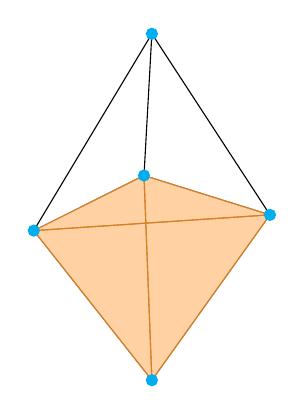
\begin{tikzpicture}

\coordinate (v2) at (0,-3.5) {};
\coordinate (v1) at (-1.5,-1.6) {};
\coordinate (v3) at (1.5,-1.4) {};
\coordinate (v4) at (0,0.9) {};
\coordinate (v5) at (-0.1,-0.9) {};

\draw[brown] (v1) -- (v2) -- (v3) -- cycle;
\draw[brown] (v5) -- (v2) -- (v3) -- cycle;
\draw[brown] (v1) -- (v5) -- (v3) -- cycle;
\draw[brown] (v1) -- (v2) -- (v5) -- cycle;

\fill[orange, opacity=0.2] (v1) -- (v2) -- (v3) -- cycle;
\fill[orange, opacity=0.2] (v5) -- (v2) -- (v3) -- cycle;
\fill[orange, opacity=0.2] (v1) -- (v5) -- (v3) -- cycle;
\fill[orange, opacity=0.2] (v1) -- (v2) -- (v5) -- cycle;
\draw (v1) -- (v4) -- (v3);
\draw (v4) -- (v5);

\filldraw[cyan] (v1) circle (2pt) ;
\filldraw[cyan] (v2) circle (2pt) ;
\filldraw[cyan] (v3) circle (2pt) ;
\filldraw[cyan] (v4) circle (2pt) ;
\filldraw[cyan] (v5) circle (2pt) ;
\end{tikzpicture}
\label{fig:example1}

\end{figure}
\end{example}


%todo: write example

\begin{definition}[Induced Map]
	Consider two complexes $K$, $L$ and a simplicial map $ f: K \to L $. We have a way to transform $f$ into a map $ f_\sharp: C_p(K) \to C_p(L) $, in this way 
	\[ c = \sum_{i=1}^n a_i \sigma_i \ \mapsto \ \sum_{i=1}^{??} a_i \tau_i  \]
	Where $ \tau_i = f(\sigma_i) $ if it has dimension $p$ or $ \tau_i =0 $ otherwise. We call $f_\sharp$ the \emph{induced map} of $f$.
\end{definition}

%todo: more examples




\end{document}